\documentclass[11pt,a4paper]{article}

%% ---------------------------------------------------------------- packages
\usepackage[utf8]{inputenc}
\usepackage[T1]{fontenc}
\usepackage[english]{babel}
\usepackage[a4paper,margin=2cm]{geometry}
\usepackage{amsmath,amssymb}
\usepackage{graphicx}
\usepackage{caption}
\usepackage{float}

\captionsetup{font=small, labelfont=bf}
\setlength{\parindent}{0pt}
\pagestyle{empty}

\begin{document}

%% ================================================================ TITLE
\begin{center}
{\Large\bfseries CFD Laboratory: The 1D Advection--Diffusion Equation\par}
\vspace{0.3em}
{\normalsize Finite-difference (FTCS) solution with Neumann and periodic boundary conditions\par}
\vspace{0.6em}
{\normalsize Ismael Mart\'in D\'iez\par}
\vspace{0.1em}
{\small Engineering Fluid Mechanics --- Aerospace Engineering, Universidad Carlos III de Madrid\par}
\vspace{0.1em}
{\small \today\par}
\end{center}
\vspace{-0.3em}
\rule{\linewidth}{0.4pt}
\vspace{0.6em}

%% The guidelines ask for two captioned graphs on a single A4 page.

\begin{figure}[H]
\centering
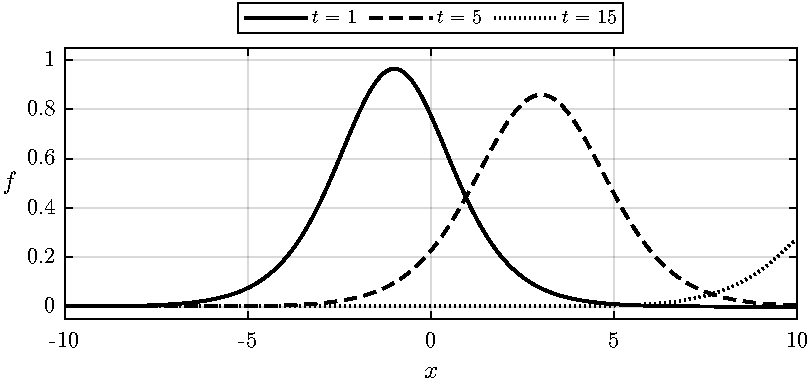
\includegraphics[width=\linewidth]{fig_neumann.pdf}
\caption{Solution $f(x,t)$ of the 1D advection--diffusion equation $\partial_t f + U\,\partial_x f = a\,\partial_x^2 f$ with Neumann boundary conditions, $\partial_x f(-10,t)=\partial_x f(10,t)=0$, at $t=1$, $t=5$ and $t=15$. Parameters: $U=1$, $a=0.1$, $k=0.5$, with initial condition $f(x,0)=\operatorname{sech}^2[k(x+2)]$. FTCS scheme with $N_x=201$ nodes ($\Delta x=0.1$) and $\Delta t=0.05$. All variables are dimensionless.}
\label{fig:neumann}
\end{figure}

\begin{figure}[H]
\centering
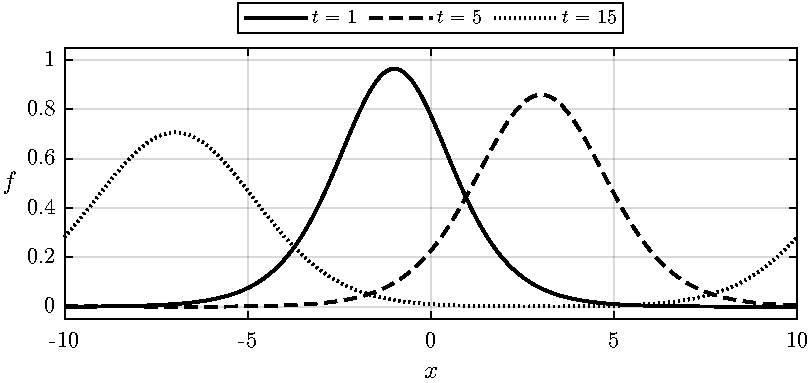
\includegraphics[width=\linewidth]{fig_periodic.pdf}
\caption{Solution $f(x,t)$ of the 1D advection--diffusion equation $\partial_t f + U\,\partial_x f = a\,\partial_x^2 f$ with periodic boundary conditions, $\partial_x f(-10,t)=\partial_x f(10,t)$, at $t=1$, $t=5$ and $t=15$. Parameters: $U=1$, $a=0.1$, $k=0.5$, with initial condition $f(x,0)=\operatorname{sech}^2[k(x+2)]$. FTCS scheme with $N_x=201$ nodes ($\Delta x=0.1$) and $\Delta t=0.05$. All variables are dimensionless.}
\label{fig:periodic}
\end{figure}

\end{document}
